\documentclass{beamer}
%
% Choose how your presentation looks.
%
% For more themes, color themes and font themes, see:
% http://deic.uab.es/~iblanes/beamer_gallery/index_by_theme.html
%
\mode<presentation>
{
  \usetheme{Madrid}      % or try Darmstadt, Madrid, Warsaw, ...
  \usecolortheme{default} % or try albatross, beaver, crane, ...
  \usefonttheme{default}  % or try serif, structurebold, ...
  \setbeamertemplate{navigation symbols}{}
  \setbeamertemplate{caption}[numbered]
}

\usepackage[english]{babel}
\usepackage[utf8x]{inputenc}

\usepackage{listings}
\usepackage{color}

\definecolor{mygreen}{rgb}{0,0.6,0}
\definecolor{mygray}{rgb}{0.5,0.5,0.5}
\definecolor{mymauve}{rgb}{0.58,0,0.82}

\lstset{
  backgroundcolor=\color{white},   % choose the background color; you must add \usepackage{color} or \usepackage{xcolor}; should come as last argument
  basicstyle=\footnotesize,        % the size of the fonts that are used for the code
  breakatwhitespace=false,         % sets if automatic breaks should only happen at whitespace
  breaklines=true,                 % sets automatic line breaking
  captionpos=b,                    % sets the caption-position to bottom
  commentstyle=\color{mygreen},    % comment style
  deletekeywords={...},            % if you want to delete keywords from the given language
  escapeinside={\%*}{*)},          % if you want to add LaTeX within your code
  extendedchars=true,              % lets you use non-ASCII characters; for 8-bits encodings only, does not work with UTF-8
  frame=single,	                   % adds a frame around the code
  keepspaces=true,                 % keeps spaces in text, useful for keeping indentation of code (possibly needs columns=flexible)
  keywordstyle=\color{blue},       % keyword style
  language=C++,                    % the language of the code
  morekeywords={*,...},            % if you want to add more keywords to the set
  numbers=left,                    % where to put the line-numbers; possible values are (none, left, right)
  numbersep=5pt,                   % how far the line-numbers are from the code
  numberstyle=\tiny\color{mygray}, % the style that is used for the line-numbers
  rulecolor=\color{black},         % if not set, the frame-color may be changed on line-breaks within not-black text (e.g. comments (green here))
  showspaces=false,                % show spaces everywhere adding particular underscores; it overrides 'showstringspaces'
  showstringspaces=false,          % underline spaces within strings only
  showtabs=false,                  % show tabs within strings adding particular underscores
  stepnumber=2,                    % the step between two line-numbers. If it's 1, each line will be numbered
  stringstyle=\color{mymauve},     % string literal style
  tabsize=2,	                   % sets default tabsize to 2 spaces
  title=\lstname                   % show the filename of files included with \lstinputlisting; also try caption instead of title
}


\title[Greedy]{Algoritmos golosos (Greedy)}
%\author{You}
%\institute{}
%\date{Date of Presentation}

\begin{document}

\begin{frame}
  \titlepage
\end{frame}

% Uncomment these lines for an automatically generated outline.
\begin{frame}{Contenidos}
  \tableofcontents
\end{frame}

\section{Algoritmos golosos}
\subsection{Qu\'e es un algoritmo goloso?}
\begin{frame}{Qu\'e es un algoritmo goloso?}
\begin{itemize}
\item
Los algoritmos golosos suelen resolver problemas de optimizaci\'on (ej: minimizar un cierto costo, o maximizar una cierta ganancia).
\item
Un algoritmo se dice goloso si toma una decisi\'on en cada paso (basada en cierto criterio), reduciendo el problema a una instancia m\'as chica.
\end{itemize}
\end{frame}
\begin{frame}{Ejemplo - problema de la moneda}
\begin{block}{Enunciado}
Dado un monto $X$ en centavos, decir la menor cantidad de monedas (de valores 100, 50, 25, 10, 5, 1) son necesarias para pagarlo exactamente (asumiendo que tengo cantidad infinita de cada tipo).
\end{block}
\pause
\begin{block}{Soluci\'on}
Tomar siempre la moneda de valor m\'as grande que no se pasa de $X$.
\end{block}
\end{frame}
\begin{frame}{Algunas consideraciones}
\begin{itemize}
\item
Las decisiones que toman los algoritmos golosos se asumen \'optimas, y no se revisan m\'as adelante.
\item
No todos los problemas admiten una soluci\'on greedy. Sin embargo, es muy com\'un creer que una idea greedy (err\'onea) funciona, pero finalmente el problema se soluciona con una t\'ecnica m\'as sofisticada.
\item
Lo ideal es demostrar que la idea greedy es correcta antes de implementarla.
\item
Sin embargo, muchas veces las ideas greedy son dif\'iciles de demostrar,  por lo que por lo general es suficiente con tener una intuici\'on de ``por qu\'e anda''.
\end{itemize}
\end{frame}
\begin{frame}{Problema de la moneda (continuaci\'on)}
\begin{itemize}
\item
Volviendo al problema de la moneda, veamos qu\'e pasa si los valores de las monedas no est\'an dados en el enunciado, sino que son input.
\end{itemize}
\begin{block}{Ejemplo}
Monedas: 1, 3, 4. Valor a pagar: 6.\\
El greedy responder\'ia [4,1,1], pero la soluci\'on \'optima es [3,3] (el greedy no funciona).
\end{block}
\begin{itemize}
\item
Como veremos m\'as adelante, este problema se resuelve mediante programaci\'on din\'amica.
\end{itemize}
\end{frame}
\subsection{Ejemplos}
\begin{frame}{M\'axima cantidad de intervalos que no se intersecan}
\url{www.spoj.com/problems/BUSYMAN/}
\begin{block}{Enunciado}
Tengo planeadas $n$ actividades. Cada una tiene un tiempo de inicio $a_i$ y un tiempo de finalizaci\'on $b_i$. Decir la mayor cantidad de actividades que puedo realizar (es decir, no se deben intersecar sus respectivos intervalos de tiempo, pero puedo empezar una actividad inmediatamente despu\'es de terminar otra).
\end{block}
\begin{figure}
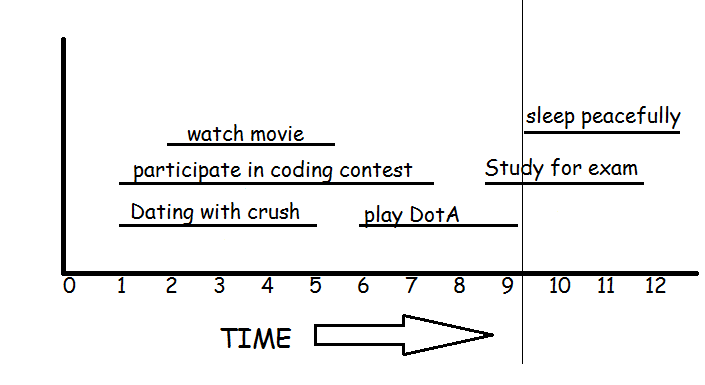
\includegraphics[width=0.6 \textwidth]{busyman}
%\caption{\label{fig:your-figure}Caption goes here.}
\end{figure}

\end{frame}

\begin{frame}{M\'axima cantidad de intervalos que no se intersecan}
\begin{itemize}
\item
Soluci\'on: Tomar siempre el intervalo que termina antes (entre los que puedo tomar).
\item
Por qu\'e anda: Supongamos que tengo una soluci\'on \'optima que no toma el que termina antes (llam\'emoslo $k$). Es f\'acil convencerse de que si reemplazo el primer intervalo de esta soluci\'on por el $k$, entonces formo otra soluci\'on \'optima, la cual contiene el $k$. Luego, existe una soluci\'on \'optima que toma la decisi\'on de agregar el $k$.
\end{itemize}

\end{frame}

\begin{frame}[fragile]{Soluci\'on - c\'odigo}
\begin{lstlisting}
int solve(int a[], int b[], int n){
	vector<pair<int,int> > intervals;
	for(int i = 0; i < n; ++i)
		intervals.push_back({b[i],a[i]});
	sort(intervals.begin(), intervals.end());
	int res = 0, last_end = -1;
	for(int i = 0; i < n; ++i){
		int start = intervals[i].second;
		int end = intervals[i].first;
		if(start >= last_end){
			res++;
			last_end = end;
		}
	}
	return res;
}
\end{lstlisting}
\end{frame}

\begin{frame}{Ganar, gustar y galantear}
\url{www.spoj.com/problems/TAP2014G/}
\begin{block}{Enunciado}
Germ\'an y Gianina organizaron un partido de f\'utbol y quieren formar los equipos eligiendo una vez cada uno qui\'en juega en su equipo. Hay $N$ (par) jugadores y cada uno tiene un valor de habilidad $a_i$.
Germ\'an elige primero, y quiere que su equipo tenga una suma de habilidades mayor que la del equipo de Gianina. Para quedar bien, en algunos turnos le deja elegir primero a Gianina. ?`Cuál es la mayor cantidad de turnos en la que puede dejar que elija Gianina de modo tal de asegurarse tener un equipo mejor que el de ella?
\end{block}
\begin{itemize}
\item
Ejemplos y soluci\'on: En pizarr\'on.
\end{itemize}
\end{frame}

\begin{frame}{Reemplazar d\'igitos minimizando suma}
\url{http://codeforces.com/contest/910/problem/C}
\begin{block}{Enunciado}
Dada una expresi\'on de la forma $s_1 + s_2 + \dots + s_n$, donde los $s_i$ son strings de caracteres entre 'a' y 'j', reemplazar cada letra por un d\'igito decimal distinto, de modo que los $s_i$ no empiecen con $0$, y se minimice el resultado de evaluar la expresi\'on. \\
Por ejemplo, si la expresi\'on es `` ab + de + aj '', una soluci\'on \'optima es $10 + 23 + 14 = 47$
\end{block}
\begin{itemize}
\item
Soluci\'on: En pizarr\'on
\end{itemize}
\end{frame}

\begin{frame}{Conclusi\'on}
\begin{itemize}
\item
No hay mucha teor\'ia o algoritmos generales detr\'as de greedy, sino que cada problema tiene su particularidad. Por eso el \'enfasis en los ejemplos.
\item
No hay otra forma de aprender greedy, m\'as que resolviendo problemas que salgan con greedy :D

\end{itemize}
\end{frame}

\end{document}

